\documentclass[10pt]{beamer}
\usetheme[
%%% option passed to the outer theme
%    progressstyle=fixedCircCnt,   % fixedCircCnt, movingCircCnt (moving is deault)
  ]{Feather}
  
% If you want to change the colors of the various elements in the theme, edit and uncomment the following lines

% Change the bar colors:
\setbeamercolor{Feather}{fg=shtred!20,bg=shtred}

% Change the color of the structural elements:
\setbeamercolor{structure}{fg=shtred}

% Change the frame title text color:
%\setbeamercolor{frametitle}{fg=blue}

% Change the normal text color background:
%\setbeamercolor{normal text}{fg=black,bg=gray!10}

%-------------------------------------------------------
% INCLUDE PACKAGES
%-------------------------------------------------------

\usepackage[utf8]{inputenc}
\usepackage[english]{babel}
\usepackage[T1]{fontenc}
\usepackage{helvet}
\usepackage{gbt7714}
\usepackage{ctex}
\setmainfont{Times New Roman}
\setCJKmainfont{SimSun}
%-------------------------------------------------------
% DEFFINING AND REDEFINING COMMANDS
%-------------------------------------------------------

% colored hyperlinks
\newcommand{\chref}[2]{
  \href{#1}{{\usebeamercolor[bg]{Feather}#2}}
}
\newcommand{\xiaosihao}{\fontsize{12pt}{18pt}\selectfont} % 小四号汉字
\newcommand{\xiaowuhao}{\fontsize{9pt}{\baselineskip}\selectfont} % 小五号汉字
%-------------------------------------------------------
% INFORMATION IN THE TITLE PAGE
%-------------------------------------------------------

\title[] % [] is optional - is placed on the bottom of the sidebar on every slide
{ % is placed on the title page
      \textbf{预测 2022 年社会消费品零售总额的损失\\基于季节性 ARIMA 模型}
}

\subtitle[预测 2022 年社会消费品零售总额的损失]
{
      \textbf{杨在洲}
}

\author[杨在洲]
{      
	yangzzh@shanghaitech.edu.cn
}



\date{\today}

%-------------------------------------------------------
% THE BODY OF THE PRESENTATION
%-------------------------------------------------------

\begin{document}

%-------------------------------------------------------
% THE TITLEPAGE
%-------------------------------------------------------

{\1% % this is the name of the PDF file for the background
\begin{frame}[plain, noframenumbering] % the plain option removes the header from the title page, noframenumbering removes the numbering of this frame only
  \titlepage % call the title page information from above
\end{frame}}


\begin{frame}{目录}{}
\tableofcontents
\end{frame}

%-------------------------------------------------------
\section{数据分析}
%-------------------------------------------------------
\subsection{数据来源}
\begin{frame}{数据来源}
\transduration{0.75}
%-------------------------------------------------------

  \begin{itemize}
    \item  采用的数据为2012年1月起至2022年4月的月度数据,来自国家统计局
    \item  选择2022年2月份以前的数据作为训练集
  \end{itemize}
\end{frame}

\subsection{季节性分解}
\begin{frame}{季节性分解}
\transduration{0.75}
%-------------------------------------------------------
  \begin{center}
    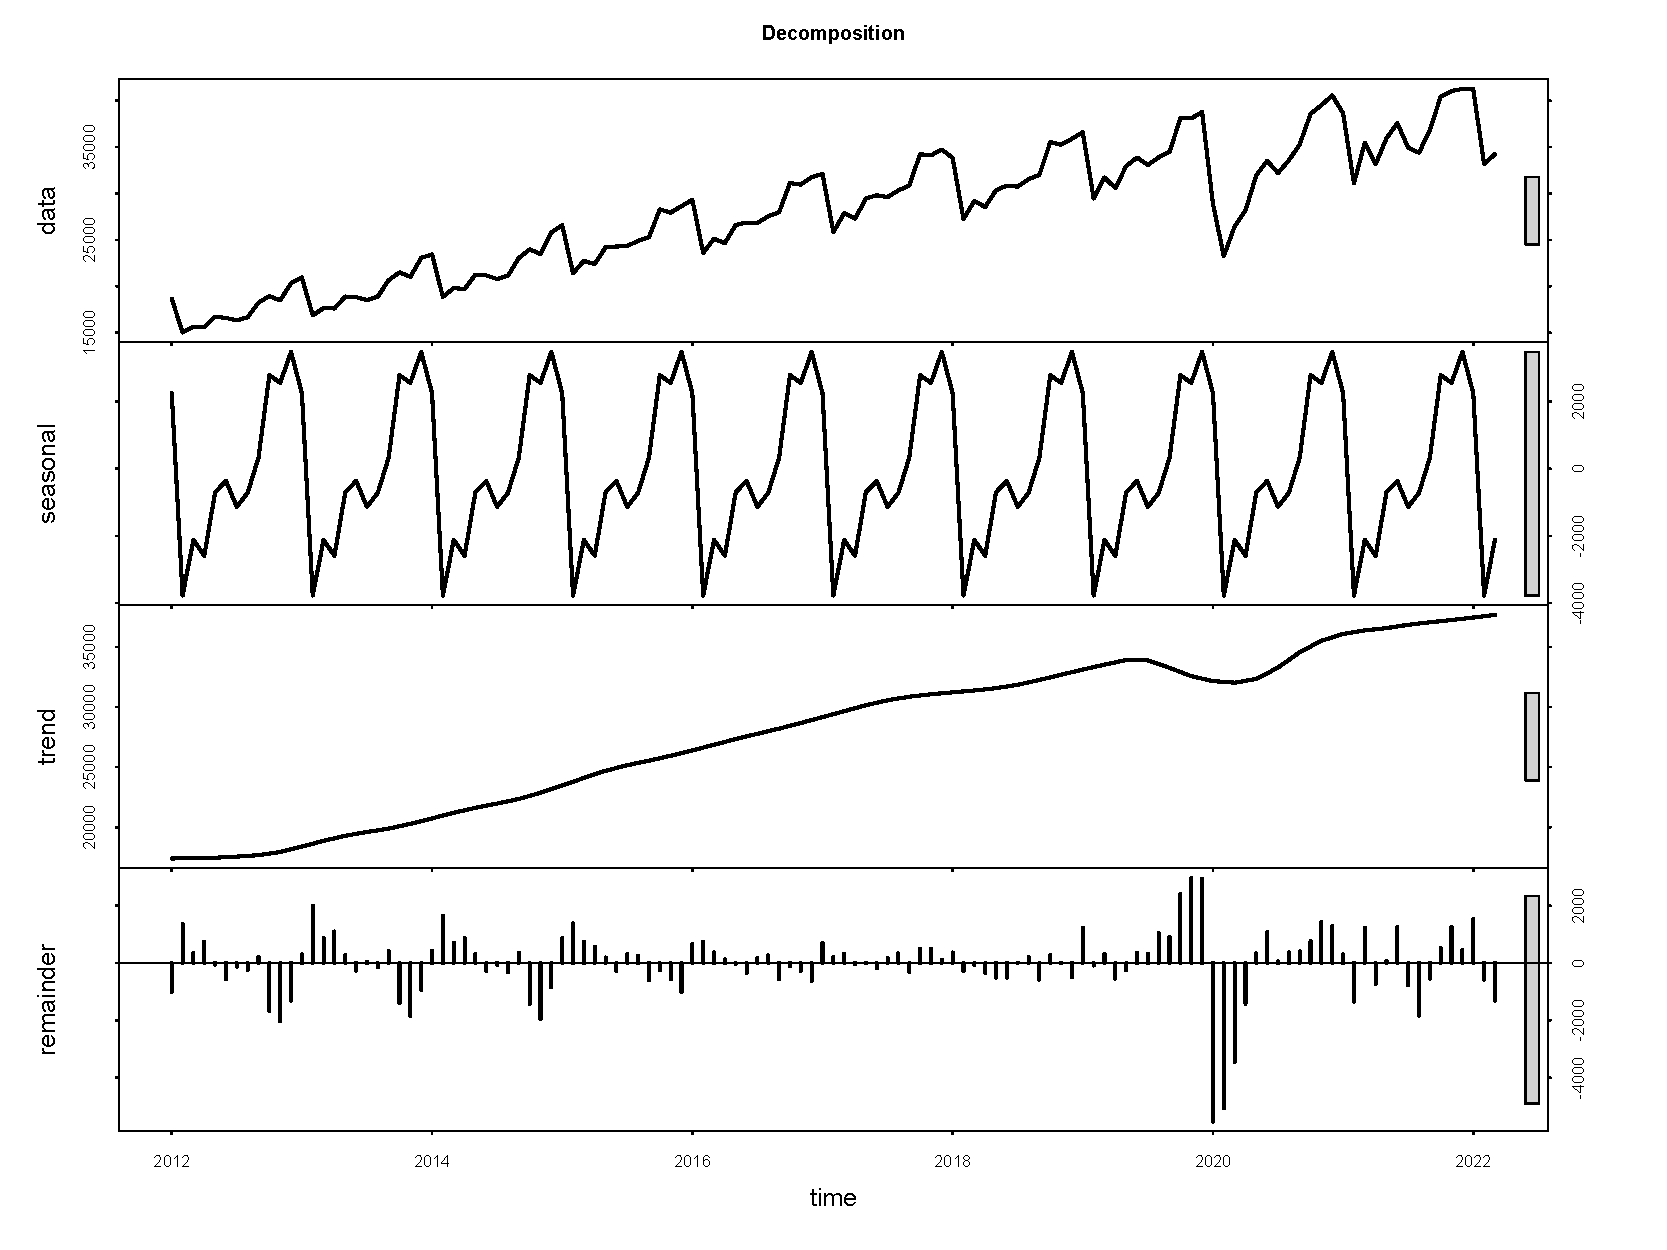
\includegraphics[width=0.8\textwidth]{figures/decompose.pdf} 
  \end{center}
  
\end{frame}


%-------------------------------------------------------
\section{建立ARIMA模型}
%-------------------------------------------------------
\subsection{数据检验}
\begin{frame}{建立ARIMA模型}{数据检验}
\transduration{0.75}

%-------------------------------------------------------

\begin{block}{数据检验}
  \begin{itemize}
    \item  数据平稳性检验
    \item  数据随机性检验
  \end{itemize}
\end{block}
\end{frame}

%-------------------------------------------------------
\begin{frame}{平稳性检验}
%-------------------------------------------------------
  \begin{block}{平稳的时间序列}
    若时间序列\(X_t\)满足如下条件:

    \begin{itemize}
      \item 均值\(E ( X_t ) = \mu \),均值\(\mu\)是与时间\(t\)无关的常数
      \item 方差\(Var(X_t) = \sigma^2\),方差\(\sigma\)是与时间\(t\)无关的常数
      \item 协方差\(Cov(X_t,X_{t+k}) = \gamma^2\),协方差只与间隔\(t\)有关  
    \end{itemize}

    则称时间序列\(X_t\)是平稳的时间序列
  \end{block}
\end{frame}
     

%--------------------------------------------------F-----
\begin{frame}{ADF检验}
%-------------------------------------------------------
  \begin{block}{ADF检验}
    \begin{equation*}
      \begin{aligned}
      &\Delta X_t = \delta X_{t-1} + \sum_{i=1}^{m}\beta_i X_{t-i} + \epsilon_t \\
      &\Delta X_t =\alpha + \delta X_{t-1} + \sum_{i=1}^{m}\beta_i X_{t-i} + \epsilon_t \\
      &\Delta X_t =\alpha +\beta_t+ \delta X_{t-1} + \sum_{i=1}^{m}\beta_i X_{t-i} + \epsilon_t
      \end{aligned}
    \end{equation*}
  \end{block}

  三个模型原假设都是\(H_0 : \delta = 0\).若拒绝\(H_0\)则为平稳序列,否则为非平稳序列。
  通过\(ADF \)临界值表判断是否接受\(H_0\)
\end{frame}

%-------------------------------------------------------
\begin{frame}{ADF检验}
%-------------------------------------------------------

  对原序列做\(ADF\)检验,得到结果如下:
  % Table generated by Excel2LaTeX from sheet 'Sheet1'
  \begin{table}[htb]
    \centering
    \caption{原时序\(X_t\)的ADF检验结果}
      \begin{tabular}{l|r}
      \multicolumn{2}{c}{ Augmented Dickey-Fuller Test} \\
      \hline
      Lag Order: & 1 \\
      Dickey-Fuller: & 0.3394\\
      P Value  & 0.7218 \\
      \end{tabular}%
    \label{tab:ADF_raw}%
  \end{table}%
  \(p>0.05\)无法拒绝原假设,原时序非平稳
\end{frame}

\begin{frame}{ADF检验}
  为去掉了原序列线性的趋势因子,对原时序\(X_t\)进行一阶差分得到\(\hat{X_t}\)
  \begin{table}[H]
  \centering
  \caption{一阶差分时序\(\hat{X_t}\)的ADF检验结果}
    \begin{tabular}{l|r}
    \multicolumn{2}{c}{ Augmented Dickey-Fuller Test} \\
    \hline
    Lag Order: & 1 \\
    Dickey-Fuller: & -7.5267\\
    P Value  & 0.01 \\
    \end{tabular}%
  \label{tab:ADF_diff}%
\end{table}%
由于\(p<0.05\)所以拒绝原假设,差分后的序列是平稳的,
\end{frame}


%-------------------------------------------------------
\begin{frame}{随机性检验}
%-------------------------------------------------------

  采用Ljung-Box检验\(\hat{X_t}\)随机性,
  假设\(H_0\):为对所有的\(k>0\),样本的自相关系数服从:
  \[\hat{\rho}_k \approx N(0,\frac{1}{n})\]
  得到的Ljung-Box检验结果为:
% Table generated by Excel2LaTeX from sheet 'Sheet1'
  \begin{table}[H]
    \centering
    \caption{Ljung-Box检验}
      \begin{tabular}{l|r}
      \multicolumn{2}{c}{Ljung-Box test} \\
      \hline
      X-squared  & \multicolumn{1}{r}{494.39} \\
      df    & \multicolumn{1}{r}{6} \\
      p-value & < 2.2e-16 \\
      \end{tabular}%
    \label{tab:Ljung-Box}%H
  \end{table}%

  由于\(p<0.05\)所以拒绝原假设,则\(\Delta X_t\)为非随机序列,可进行下一步建模。
\end{frame}
%-------------------------------------------------------
\subsection{参数估计}
%-------------------------------------------------------
\begin{frame}{ARIMA模型}
\begin{block}{ARIMA模型}
  给定一个差分\(d\)阶的时间序列\(y'_t\),\(ARIMA(p,d,q)\)模型如下:

  \[y'_t=c+\sum_{i=1}^p{\phi_i y'_{t-i}}+\sum_{i=1}^q{\theta_i\varepsilon_{t-i}}+\varepsilon_t \]

  或者写为\[(1-\phi_1B - \cdots - \phi_p B^p)  (1-B)^d y_{t} = c + (1 + \theta_1 B + \cdots + \theta_q B^q)\varepsilon_t\]

  其中\(\varepsilon_t\)是白噪声序列, \(p\)是自回归的阶数,\(q\)是移动平均的阶数。
\end{block}
\end{frame}

\begin{frame}{自相关系数}
  \begin{block}{自相关系数ACF}
    \[\rho_h = \rho(y_t,y_{t+k}) =\frac{Cov(y_t,y_{t+k})}{\sigma_t \sigma_{t+k}}\]
  \end{block}

  平稳序列的自相关函数\(ACF\)与时间间隔\(k\)有关,\(ACF\)图显示了\(y_t\)与\(y_{t-k}\)之间相关性,
  可通过\(ACF\)相关系数决定\(q\).
\end{frame}

\begin{frame}{偏自相关系数}
  \begin{block}{偏自相关系数PACF}
    在计算相关性时移除了中间变量\(y_{t-1},
    y_{t-2},\cdots,y_{t-k+1}\)的间接影响,直接得到\(y_t\)与\(y_{t-k}\)之间的相关性,
    通过\(PACF\)估计\(P\)值
  \end{block}
\end{frame}

\begin{frame}{参数估计}
  根据ACF和PACF图的拖尾情况选取合适的参数p,q:
  \begin{center}
    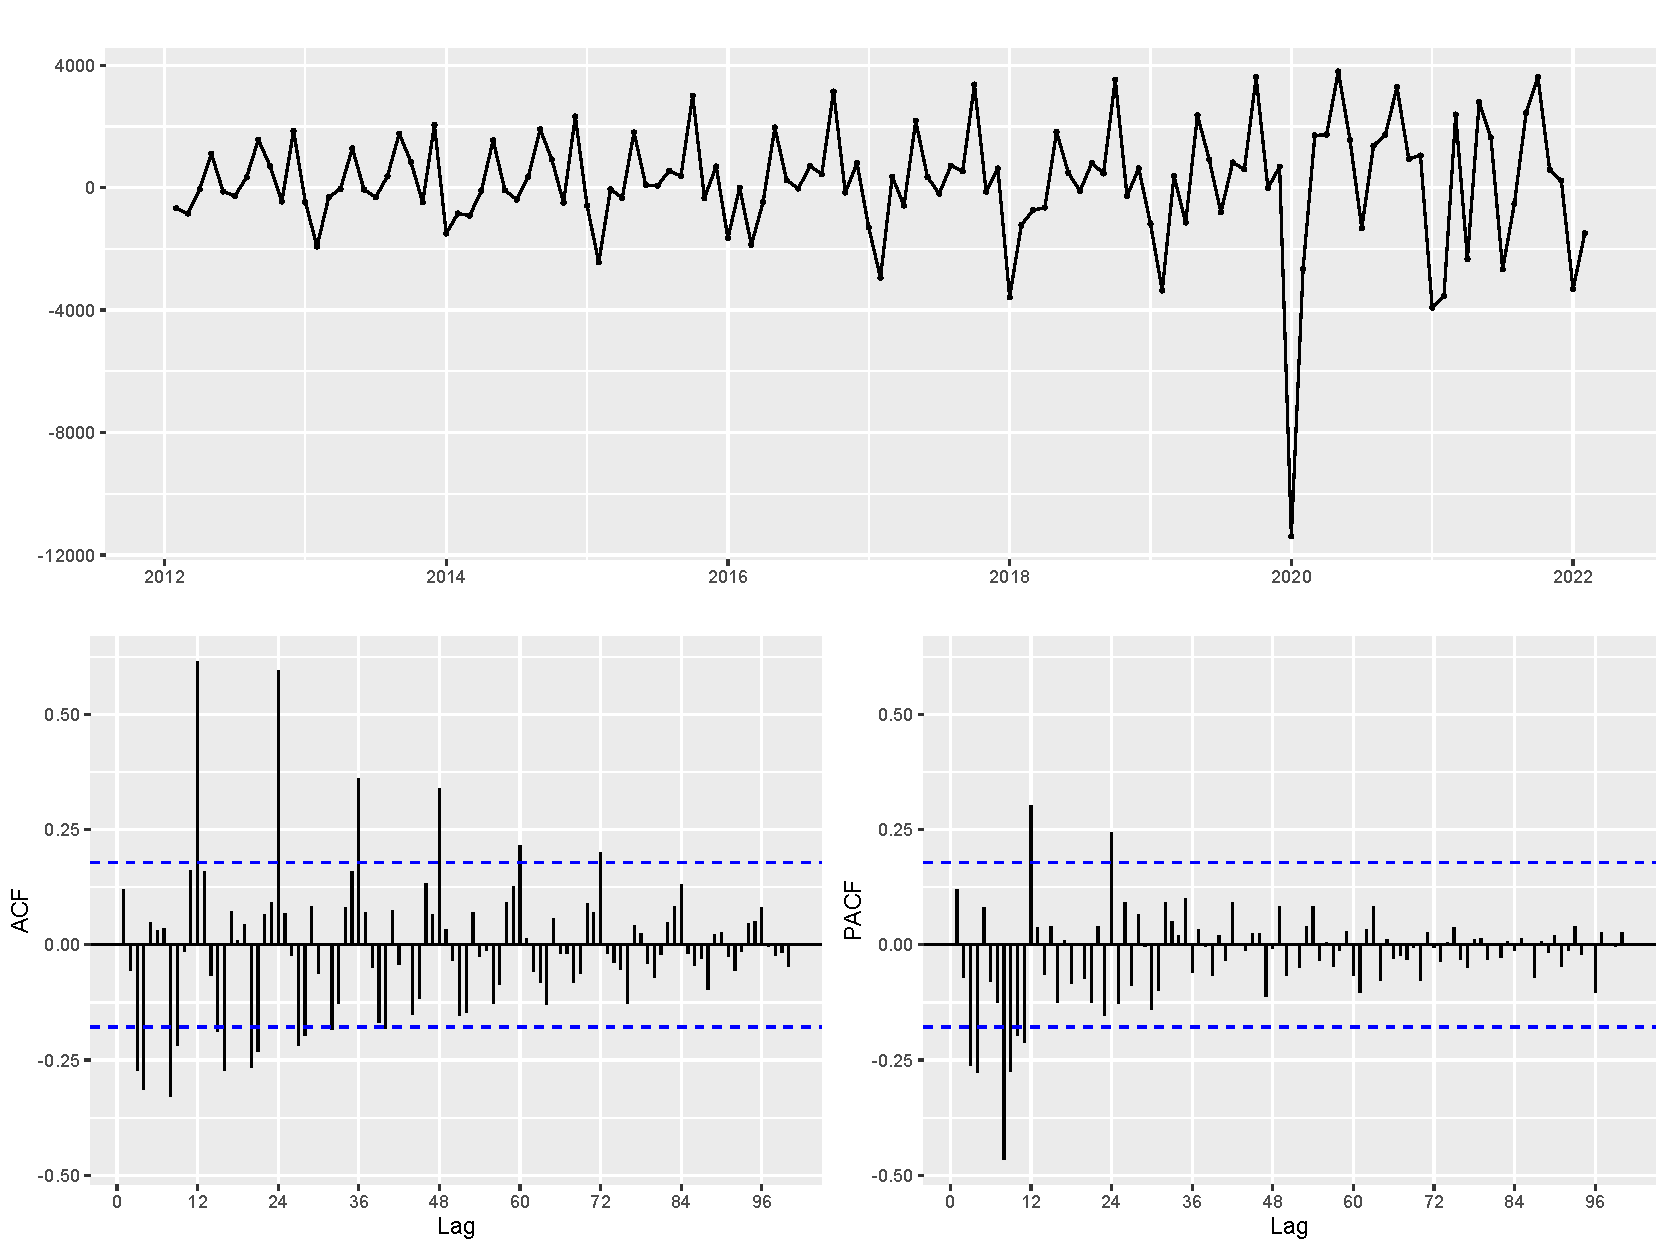
\includegraphics[width=0.8\textwidth]{figures/acf_pacf.pdf}
  \end{center}   
\end{frame}
%-------------------------------------------------------
%-------------------------------------------------------
\begin{frame}{季节性ARIMA模型}
  \begin{block}{季节性ARIMA模型}
    将一阶差分序列\(\Delta X_t\)进行分解,写成季节,部分与非季节部分的乘积

    \begin{center}
      ARIMA\;\;\;\;	\((p, d, q)\)	\;\;\;\;\; \((P, D, Q)_{m}\) \label{Season_decompose}
    \end{center}
    
    例如对于\(ARIMA(1,1,1)(1,1,1)_m\)模型:
    \[(1 - \phi_{1}B)~(1 - \Phi_{1}B^{12})~(1 - B)~(1 - B^{12})y_{t} = (1 + \theta_{1}B)~ (1 + \Theta_{1}B^{12})\varepsilon_{t}\]
  \end{block}
\end{frame}

\begin{frame}{季节性差分}
  \begin{block}{季节性差分}
    观测周期为12个月,为先消除季节型波动,对\(\Delta X_t\)再进行差分
    \[X'_{t} = \Delta X_t-\Delta X_{t-12}\]
  \end{block}
\end{frame}

\begin{frame}{季节性差分}
  得到序列\(X'_t\)的自相关图:
  \begin{center}
    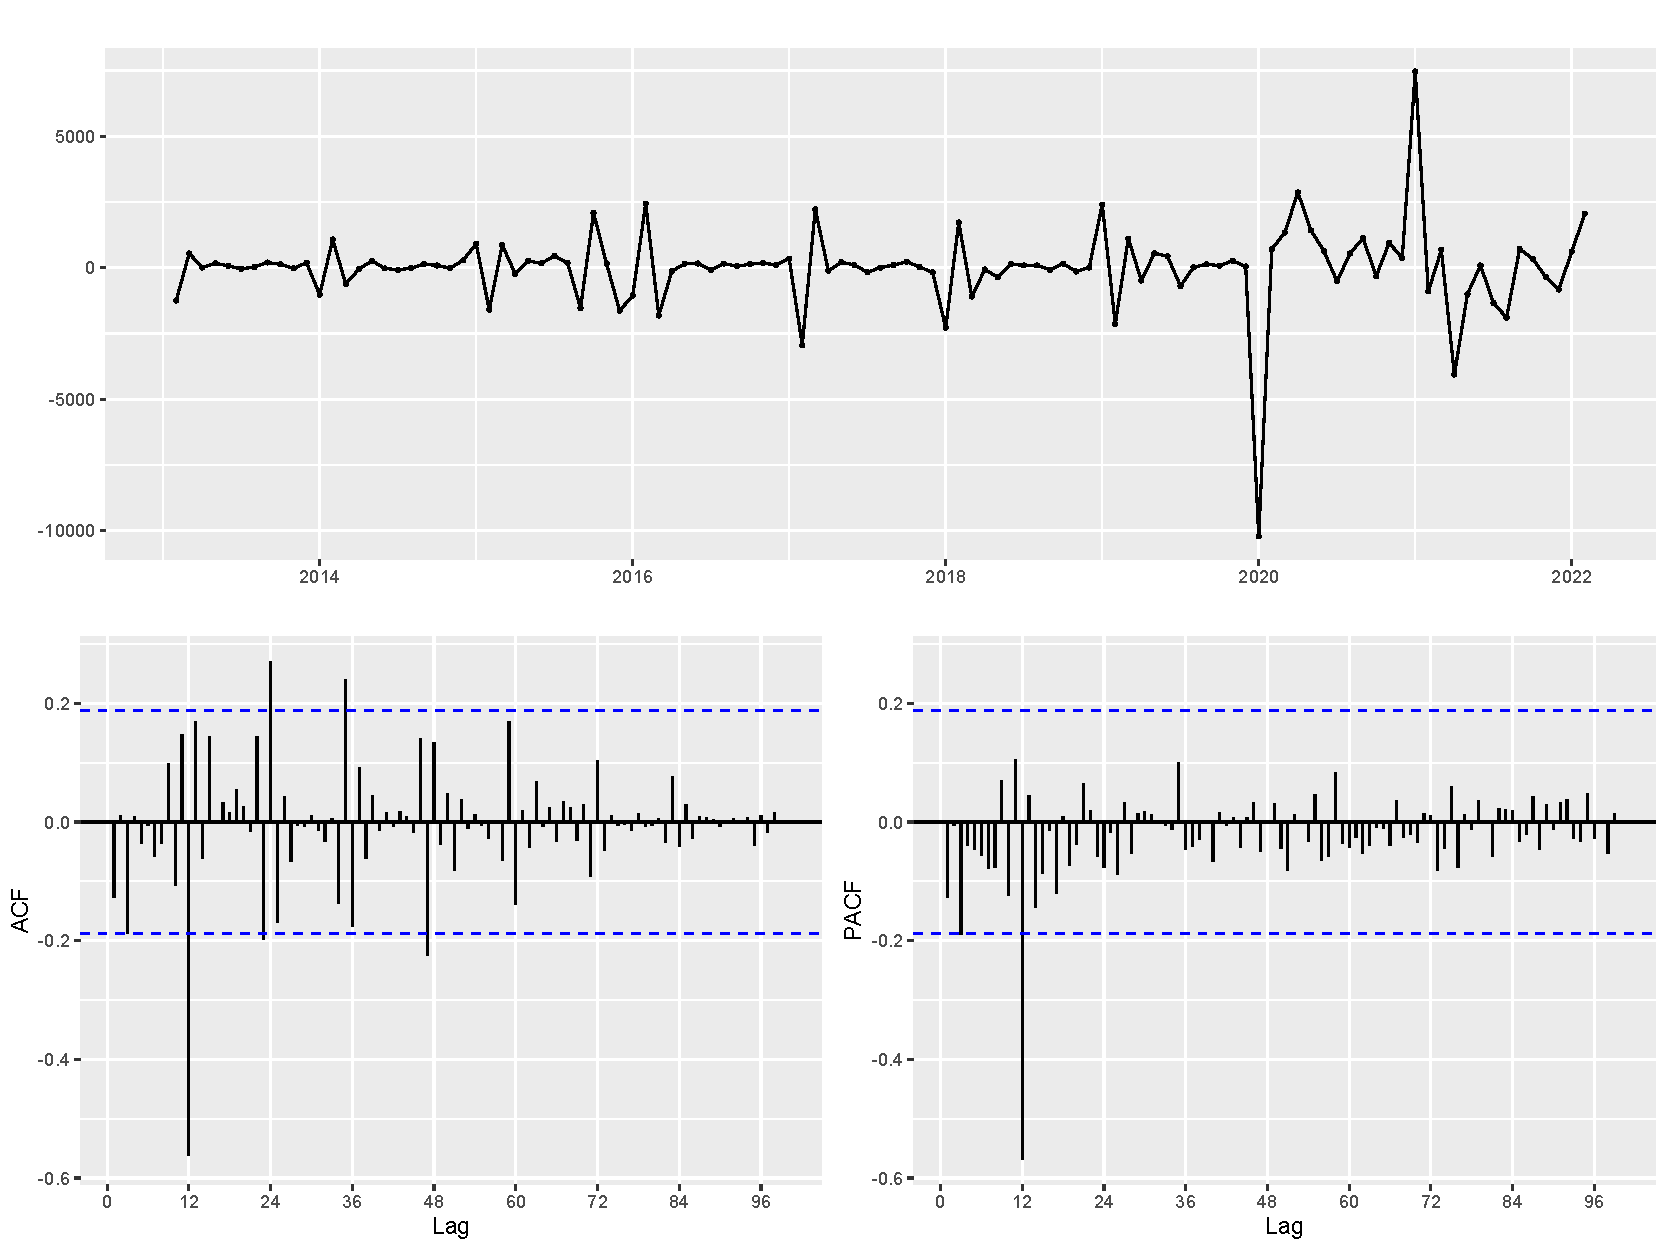
\includegraphics[width=0.8\textwidth]{figures/Season_diff.pdf}
  \end{center}   
\end{frame}

\begin{frame}{参数估计}
  \begin{block}{参数确定}
    \begin{itemize}
      \item 可确定季节部分相应系数\(P=1 , Q=1\)
      \item 非季节部分的ACF和PACF图较难判断产生拖尾的临界点
    \end{itemize}
  \end{block}
\end{frame}



\begin{frame}
  \frametitle{模型选择}
  利用AIC,AICc,BIC准则定量的确定在何种系数下的模型最优
  \begin{block}{AIC(赤池信息准则)}
    \[\text{AIC} = -2log(L) + 2(p+q+k+1)\]
    \xiaowuhao{其中\(L\)数据的似然函数,最后一项为参数个数(包含了余项的方差)\(k=0\)若\(c=0\),\(k=1\)若\(c\neq0\)
    对于ARIMA模型而言,修正过的AIC值可以被表示为:}
    \[\text{AICc} = \text{AIC} + \frac{2(p+q+k+1)(p+q+k+2)}{T-p-q-k-2}\]
  \end{block}
\end{frame}


\begin{frame}{模型选择}
    \begin{block}{AICc(赤池信息量准则)}
    \[\text{AICc} = \text{AIC} + \frac{2(p+q+k+1)(p+q+k+2)}{T-p-q-k-2}\]
  \end{block}
  \begin{block}{BIC(贝叶斯信息准则)}
    \[\text{BIC} = \text{AIC} + [\log(T)-2](p+q+k+1)\]
  \end{block}
\end{frame}

\begin{frame}{模型选择}
  通过枚举p,q的值得到相应模型AIC,AICc,BIC如下:
  \begin{table}[htbp]
    \centering
      \begin{tabular}{c|ccc}
      相应的ARIMA模型 & AIC   & AICc  & BIC \\
      \hline
      (0,1,0)(1,1,1)[12] & 1876.32 & 1876.55 & 1884.4 \\
      (0,1,1)(1,1,1)[12] & 1878.32 & 1878.7 & 1889.08 \\
      (0,1,2)(1,1,1)[12] & 1877.96 & 1878.54 & 1891.41 \\
      (0,1,3)(1,1,1)[12]  & 1876.22 & 1877.04 & 1892.36 \\
      (1,1,1)(1,1,1)[12] & 1880.27 & 1880.86 & 1893.73 \\
      (1,1,2)(1,1,1)[12] & 1873.59 & 1874.41 & 1889.74 \\
      (1,1,3)(1,1,1)[12] & 1875.51 & 1876.62 & 1894.35 \\
      (2,1,1)(1,1,1)[12] & 1873.53 & 1874.36 & 1889.68 \\
      (2,1,2)(1,1,1)[12] & 1875.02 & 1876.13 & 1893.86 \\
      (3,1,0)(1,1,1)[12] & 1879.02 & 1879.84 & 1895.16 \\
      (3,1,1)(1,1,1)[12] & 1875.53 & 1876.64 & 1894.37 \\
      (3,1,2)(1,1,1)[12] & 1876.98 & 1878.79 & 1901.2 \\
      \end{tabular}%
    \label{choose optimal models}%
  \end{table}%
\end{frame}

\subsection{残差检验}

\begin{frame}{残差检验}
  从表\ref{choose optimal models}中看出,ARIMA\((2,1,1)(1,1,1)_{12}\)是最优的ARIMA模型。
  对残差\(\epsilon_t\)做Ljung-Box test检验:

  \begin{table}[H]
    \centering
    \caption{残差\(Ljung-Box\)检验结果}
      \begin{tabular}{l|l}
      \multicolumn{2}{c}{Ljung-Box test} \\
      \hline
      df    & \multicolumn{1}{r}{19} \\
      p-value & 0.90 \\
      \end{tabular}%
    \label{Ljung-Box of Residuals}%H
  \end{table}%

  \(p>0.05\)无法拒绝原假设,所得残差为白噪声序列,残差之间不存在自相关性。
\end{frame}

\begin{frame}{残差检验}
  并且得到的残差图\ref{Redsiduals},残差基本符合正态分布要求:
  \begin{figure}[H] %H为当前位置,!htb为忽略美学标准,htbp为浮动图形
  \centering %图片居中
  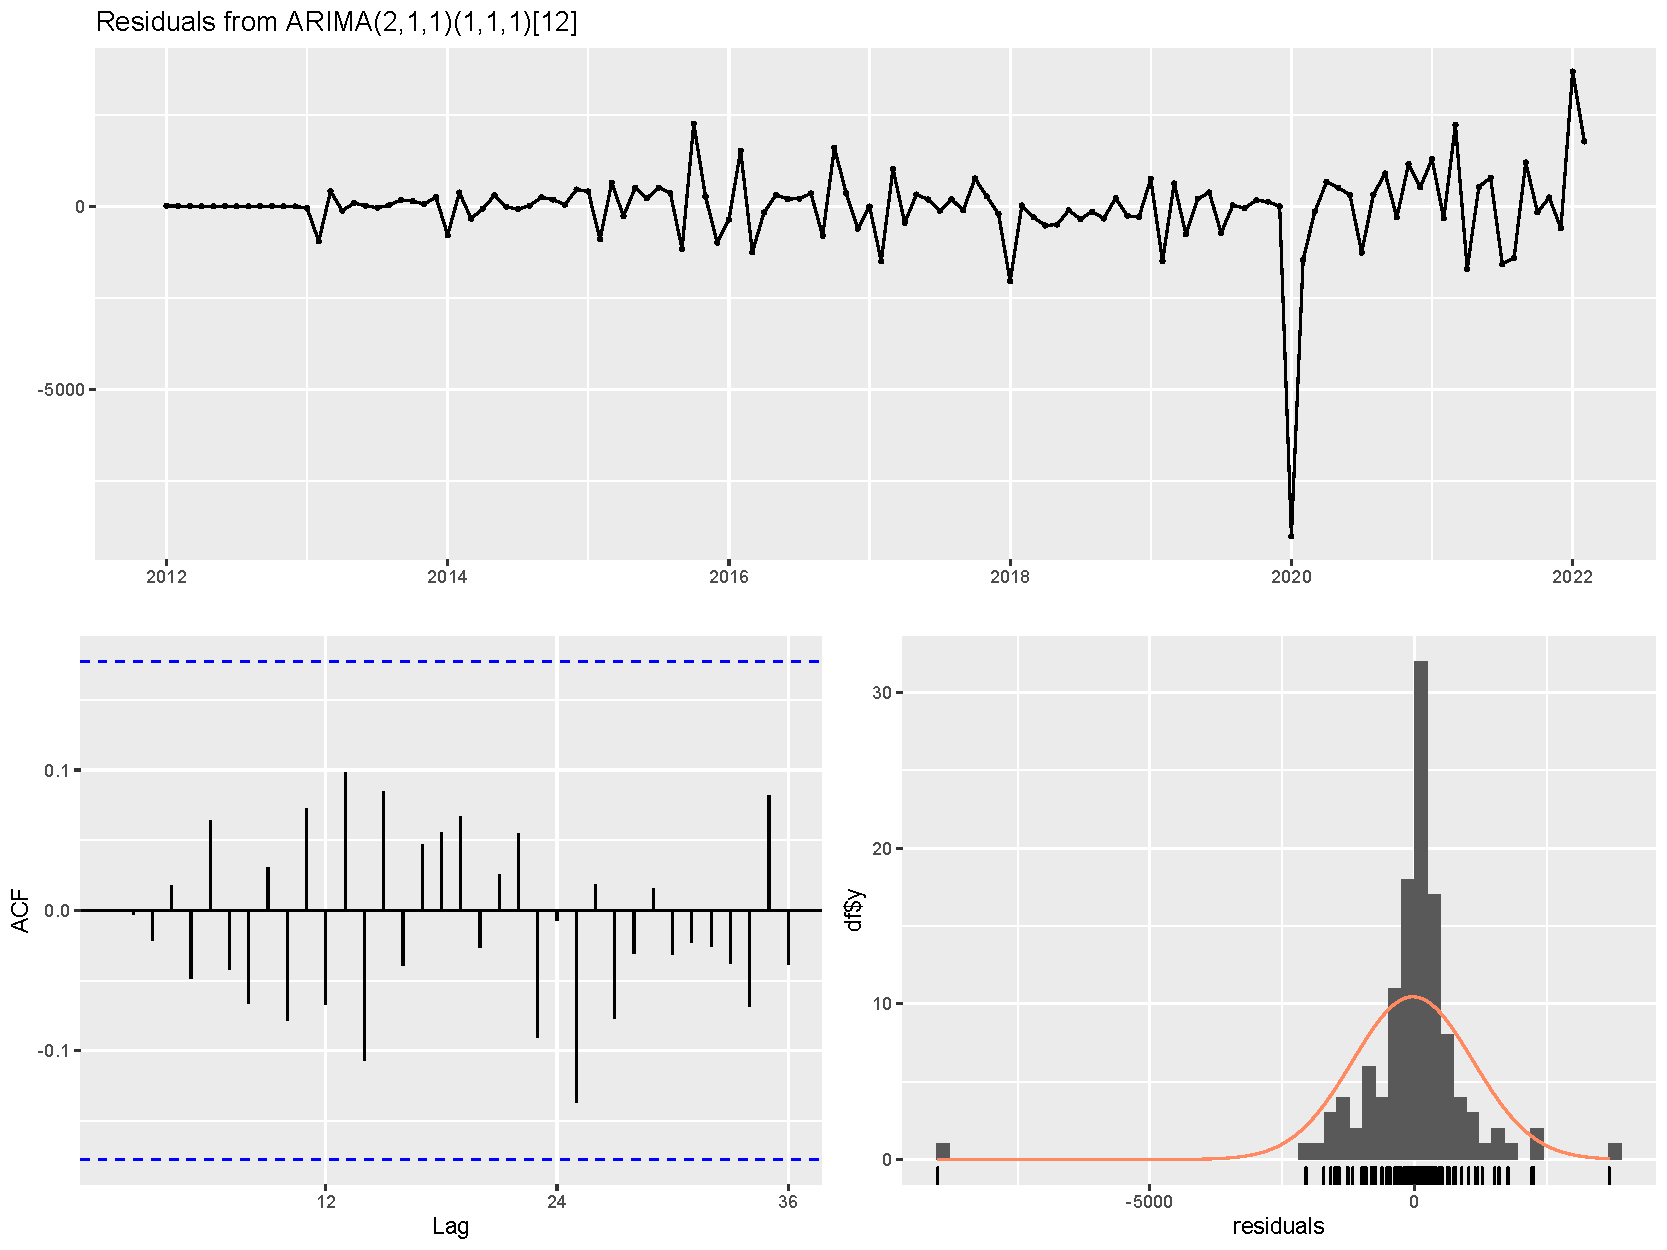
\includegraphics[width=0.7\textwidth]{figures/Residuals.pdf} %插入图片,[]中设置图片大小,{}中是图片文件名
  \caption{\(ARIMA(2,1,1)(1,1,1)_{12}\)的残差图} %最终文档中希望显示的图片标题
  \label{Redsiduals} %用于文内引用的标签
  \end{figure} 
\end{frame}

\begin{frame}
  \frametitle{残差检验}
  为进一步说明,绘出正态Q-Q图

  \begin{figure}[H] %H为当前位置,!htb为忽略美学标准,htbp为浮动图形
    \centering %图片居中
    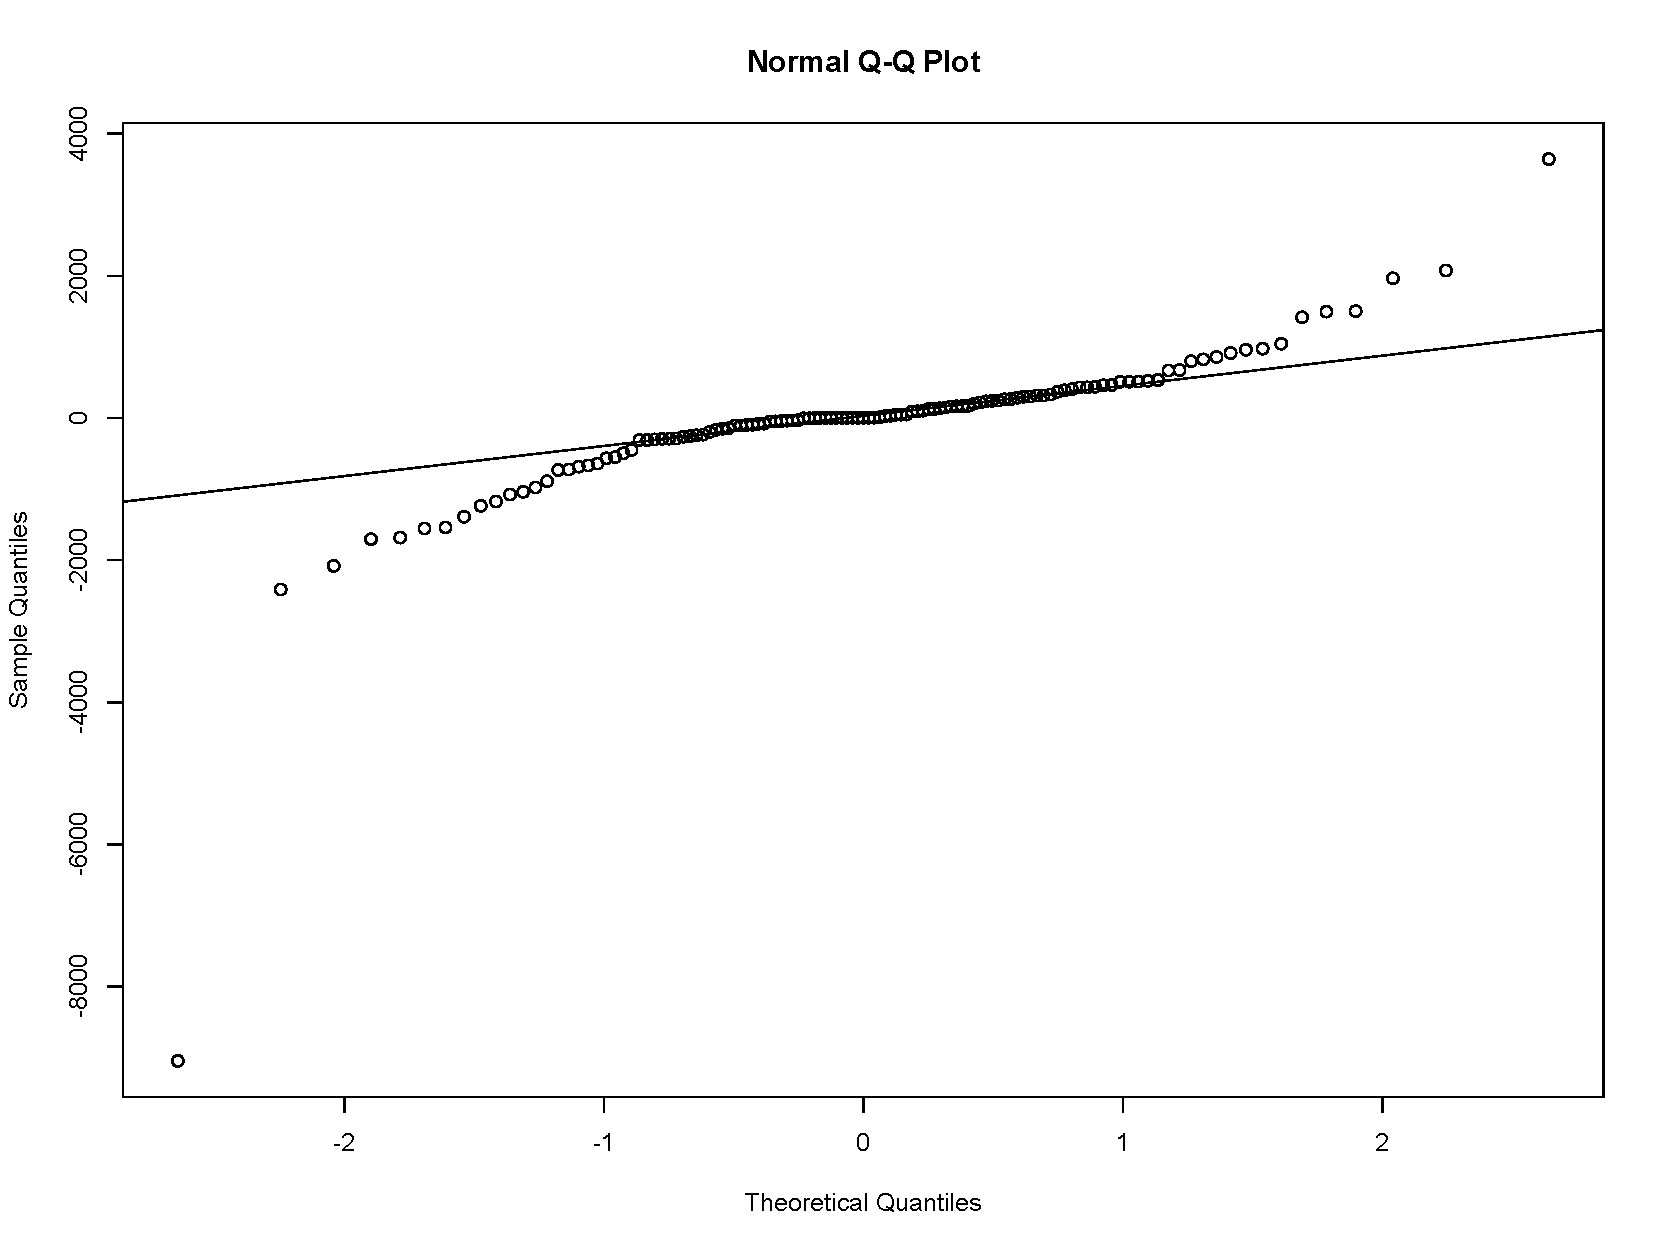
\includegraphics[width=0.7\textwidth]{figures/Q-Qplot.pdf} %插入图片,[]中设置图片大小,{}中是图片文件名
    \caption{\small{ARIMA\((2,1,1)(1,1,1)_{12}\)的残差Q-Q图}} %最终文档中希望显示的图片标题
    \label{Q-Qplot} %用于文内引用的标签
  \end{figure} 
\end{frame}

\subsection{未受疫情干预的预测}

\begin{frame}{预测}
  \begin{figure}[htbp] %H为当前位置,!htb为忽略美学标准,htbp为浮动图形
    \centering %图片居中
    \begin{minipage}[t]{0.48\textwidth}
      \centering
      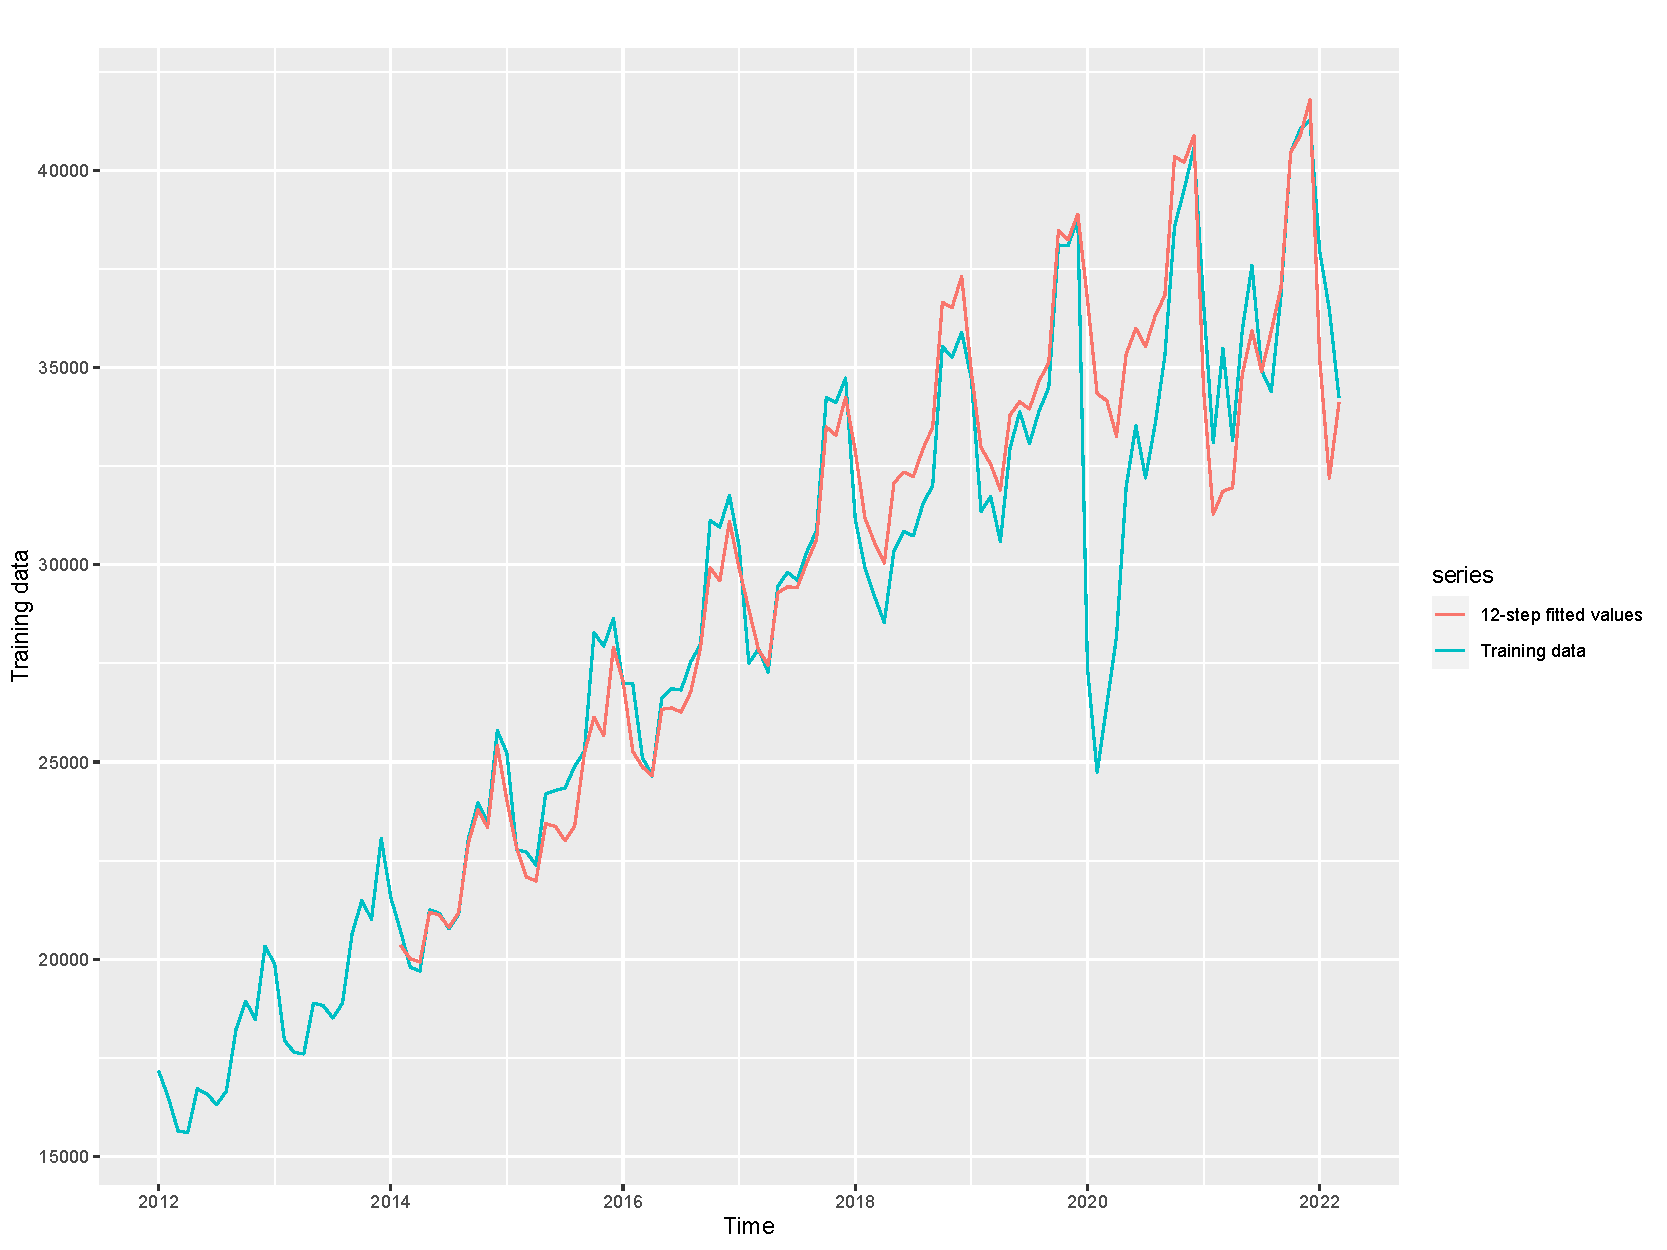
\includegraphics[width=1\textwidth]{figures/training_forecast.pdf} %插入图片,[]中设置图片大小,{}中是图片文件名
      \caption{\xiaowuhao{ARIMA模型得到的12步拟合值}} %最终文档中希望显示的图片标题
      \label{traning_forecast} %用于文内引用的标签
    \end{minipage}
    \begin{minipage}[t]{0.48\textwidth}
      \centering %图片居中
      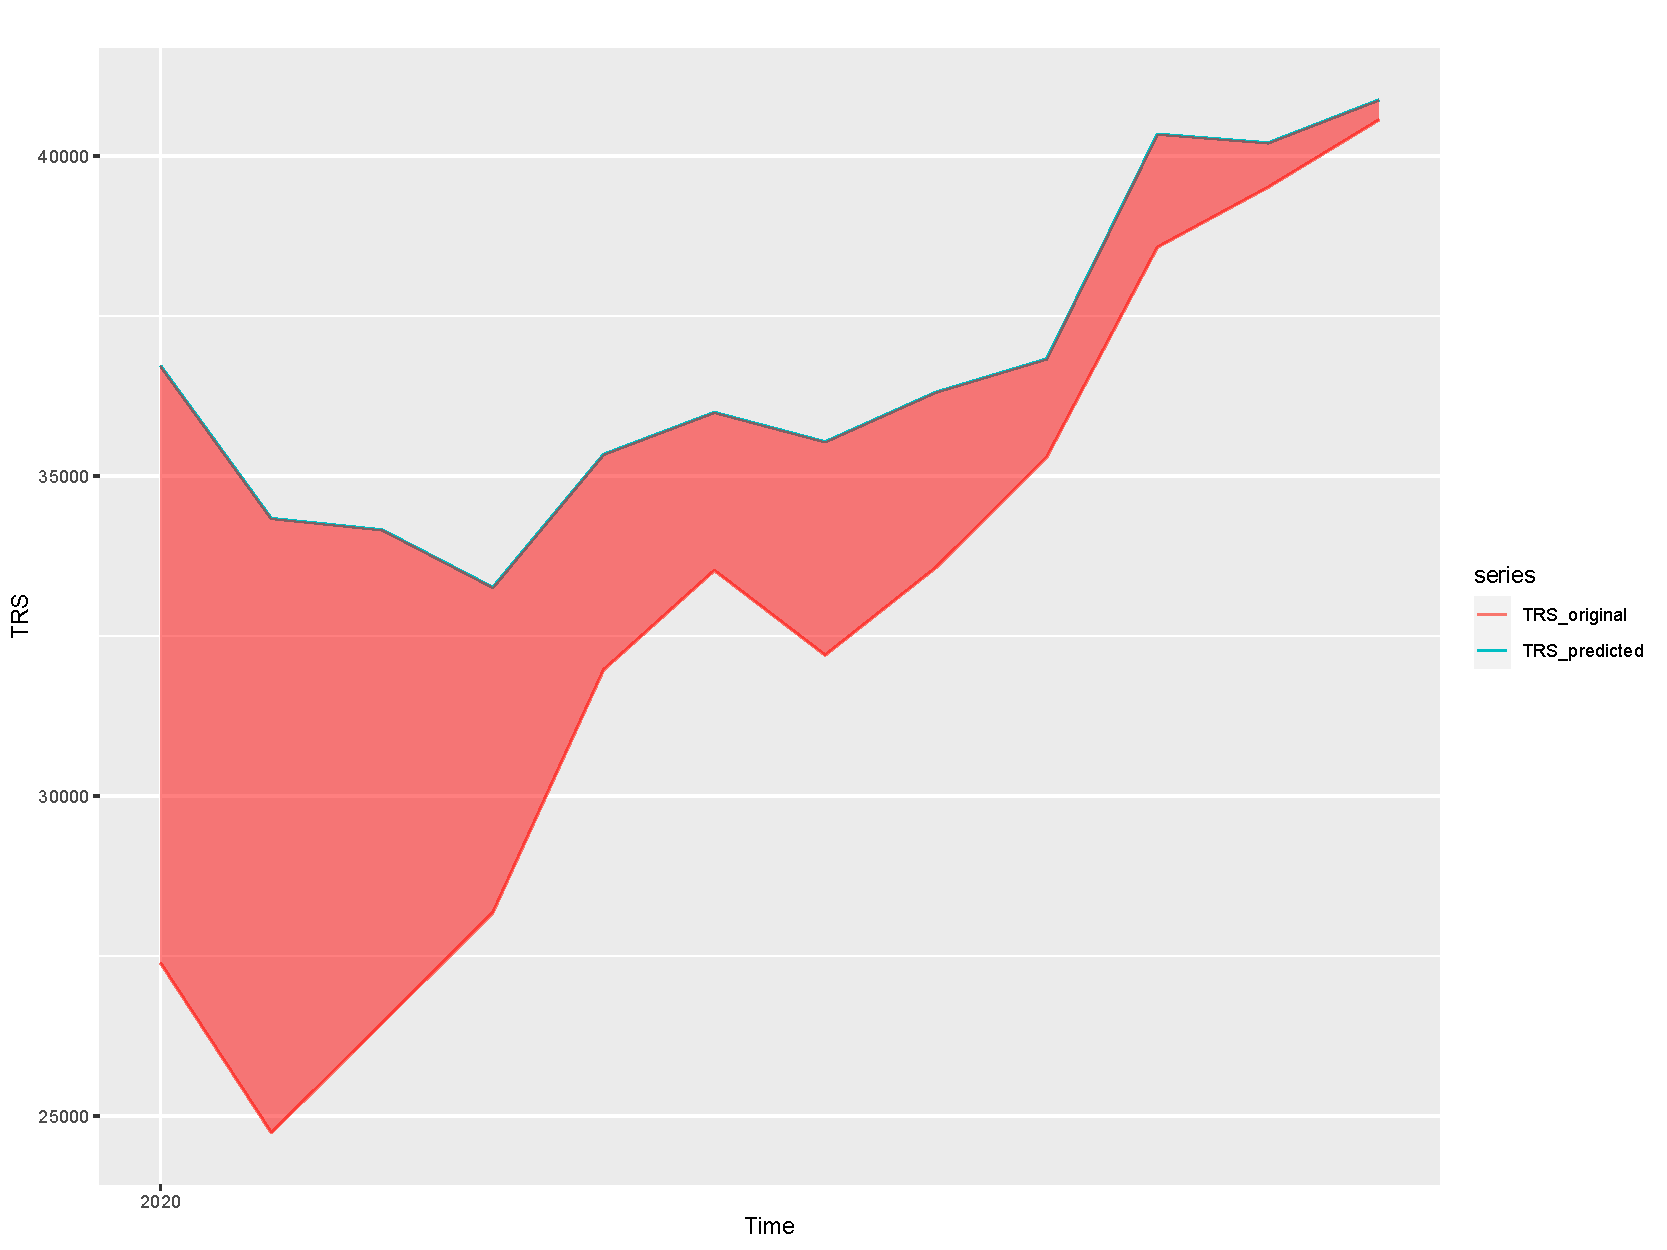
\includegraphics[width=1\textwidth]{figures/trs_2020.pdf} %插入图片,[]中设置图片大小,{}中是图片文件名
      \caption{\xiaowuhao{2020年社会消费品零售总额的损失}} %最终文档中希望显示的图片标题
      \label{trs_2020} %用于文内引用的标签
    \end{minipage}
  \end{figure} 
\end{frame}


\section{干预分析模型的建立}

\subsection{参数估计}
\begin{frame}{干预分析}
  \begin{block}{持续性干预变量}
    \[S_t^T = \begin{cases}
      0& \text{疫情发生前 t<T}\\
      1& \text{疫情发生后 t>=T}
    \end{cases}\]
  \end{block}
  \begin{block}{干预分析模型}
    设\(\omega\)为干预未知的干预系数,\(Z_t\)为疫情发生后所产生的损失的时间序列,通过一阶差分获得平稳序列,
    则干预后的模型可写为
    \[Z_t = \delta Z_{t-1} + \omega\]
  \end{block}
\end{frame}

\begin{frame}{干预模型}
  用最小二乘法的到参数的估计值,\(\delta =0.7328 , \omega =  72.1654 \)
  绘出回归拟合图像和残差图如下, 残差符合正态分布要求, 且通过Ljung-Box检验。:
  \begin{figure}[H] %H为当前位置,!htb为忽略美学标准,htbp为浮动图形
    \centering %图片居中
    \begin{minipage}[t]{0.48\textwidth}
      \centering
      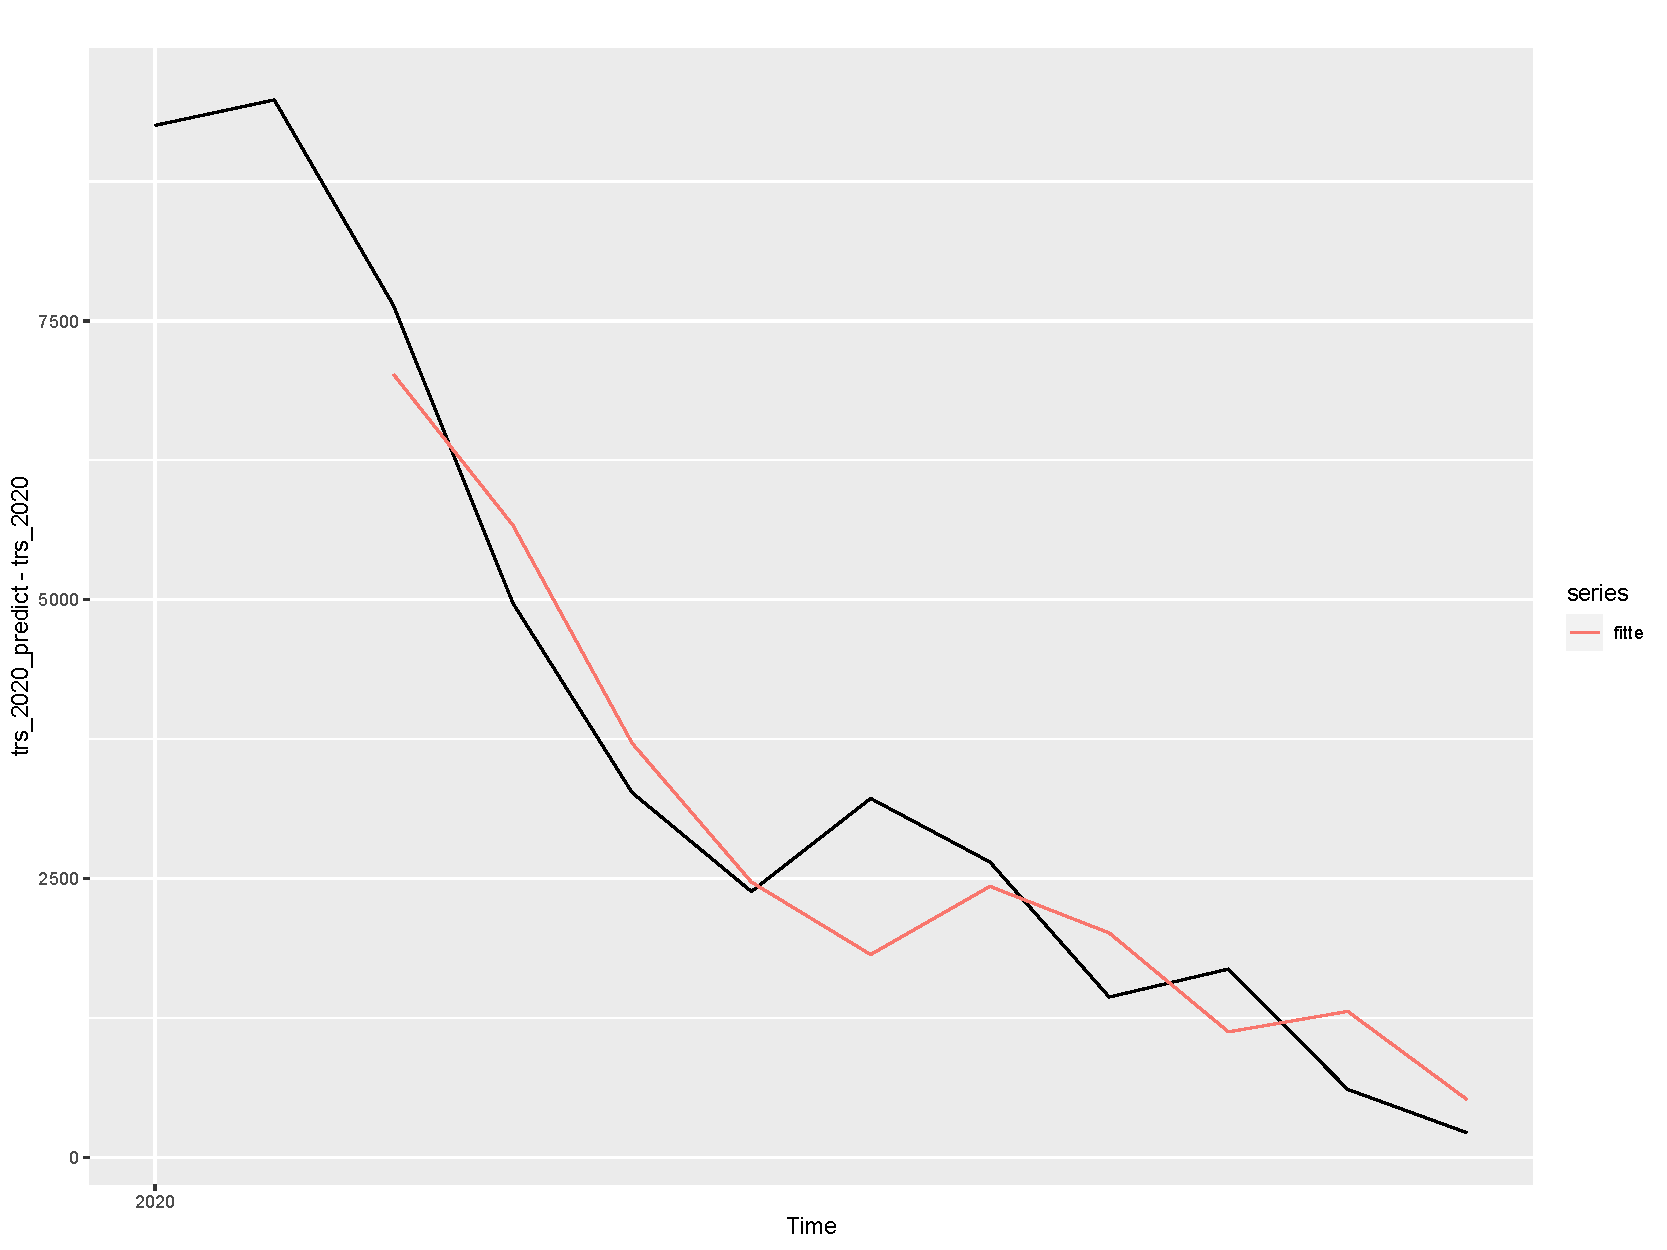
\includegraphics[width=1\textwidth]{figures/fitted_loss_2020.pdf} %插入图片,[]中设置图片大小,{}中是图片文件名
      \caption{2020年社会消费品零售总额的损失图(红色为回归结果)} %最终文档中希望显示的图片标题
      \label{fitted_loss_2020} %用于文内引用的标签
    \end{minipage}
    \begin{minipage}[t]{0.48\textwidth}
      \centering %图片居中
      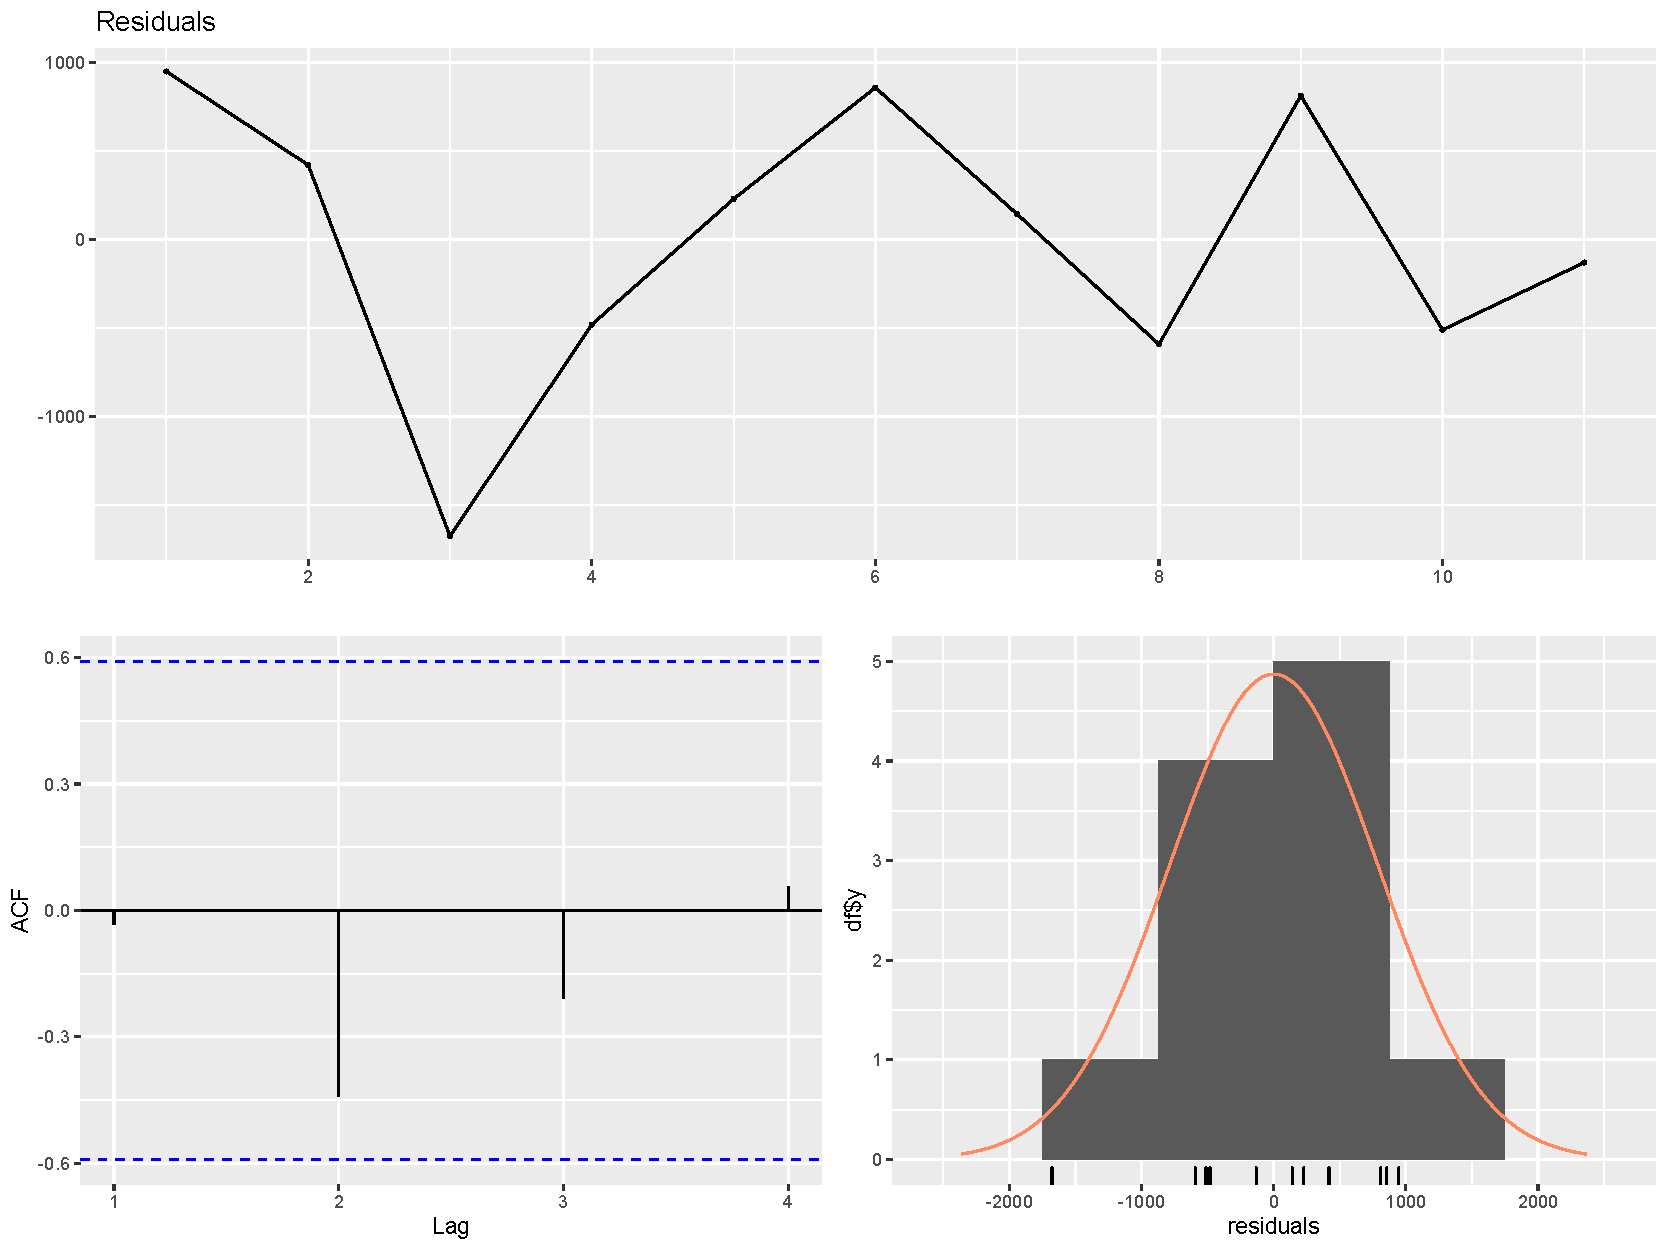
\includegraphics[width=1\textwidth]{figures/loss_model_resi.pdf} %插入图片,[]中设置图片大小,{}中是图片文件名
      \caption{回归结果的残差图} %最终文档中希望显示的图片标题
      \label{loss_model_resi} %用于文内引用的标签
    \end{minipage}
  \end{figure} 
\end{frame}

\subsection{预测结果}
\begin{frame}{预测}
  \begin{table}[H]
    \centering
    \caption{2022年3月起社会消费品零售总额的损失(单位:亿元)}
    \resizebox{\textwidth}{!}{
      \begin{tabular}{ccccccccccc}
      月份    & 3     & 4     & 5     & 6     & 7     & 8     & 9     & 10    & 11    & 12 \\
      \hline
      损失    & 3924 & 8587 & 6364 & 4735 & 3542 & 2667 & 2026 & 1557 & 1213 & 961 \\
      \end{tabular}}%
    \label{loss_2020_table}%
  \end{table}%
\end{frame}

\begin{frame}{预测}
  \begin{figure}[H] %H为当前位置,!htb为忽略美学标准,htbp为浮动图形
    \centering %图片居中
    \begin{minipage}[t]{0.48\textwidth}
      \centering
      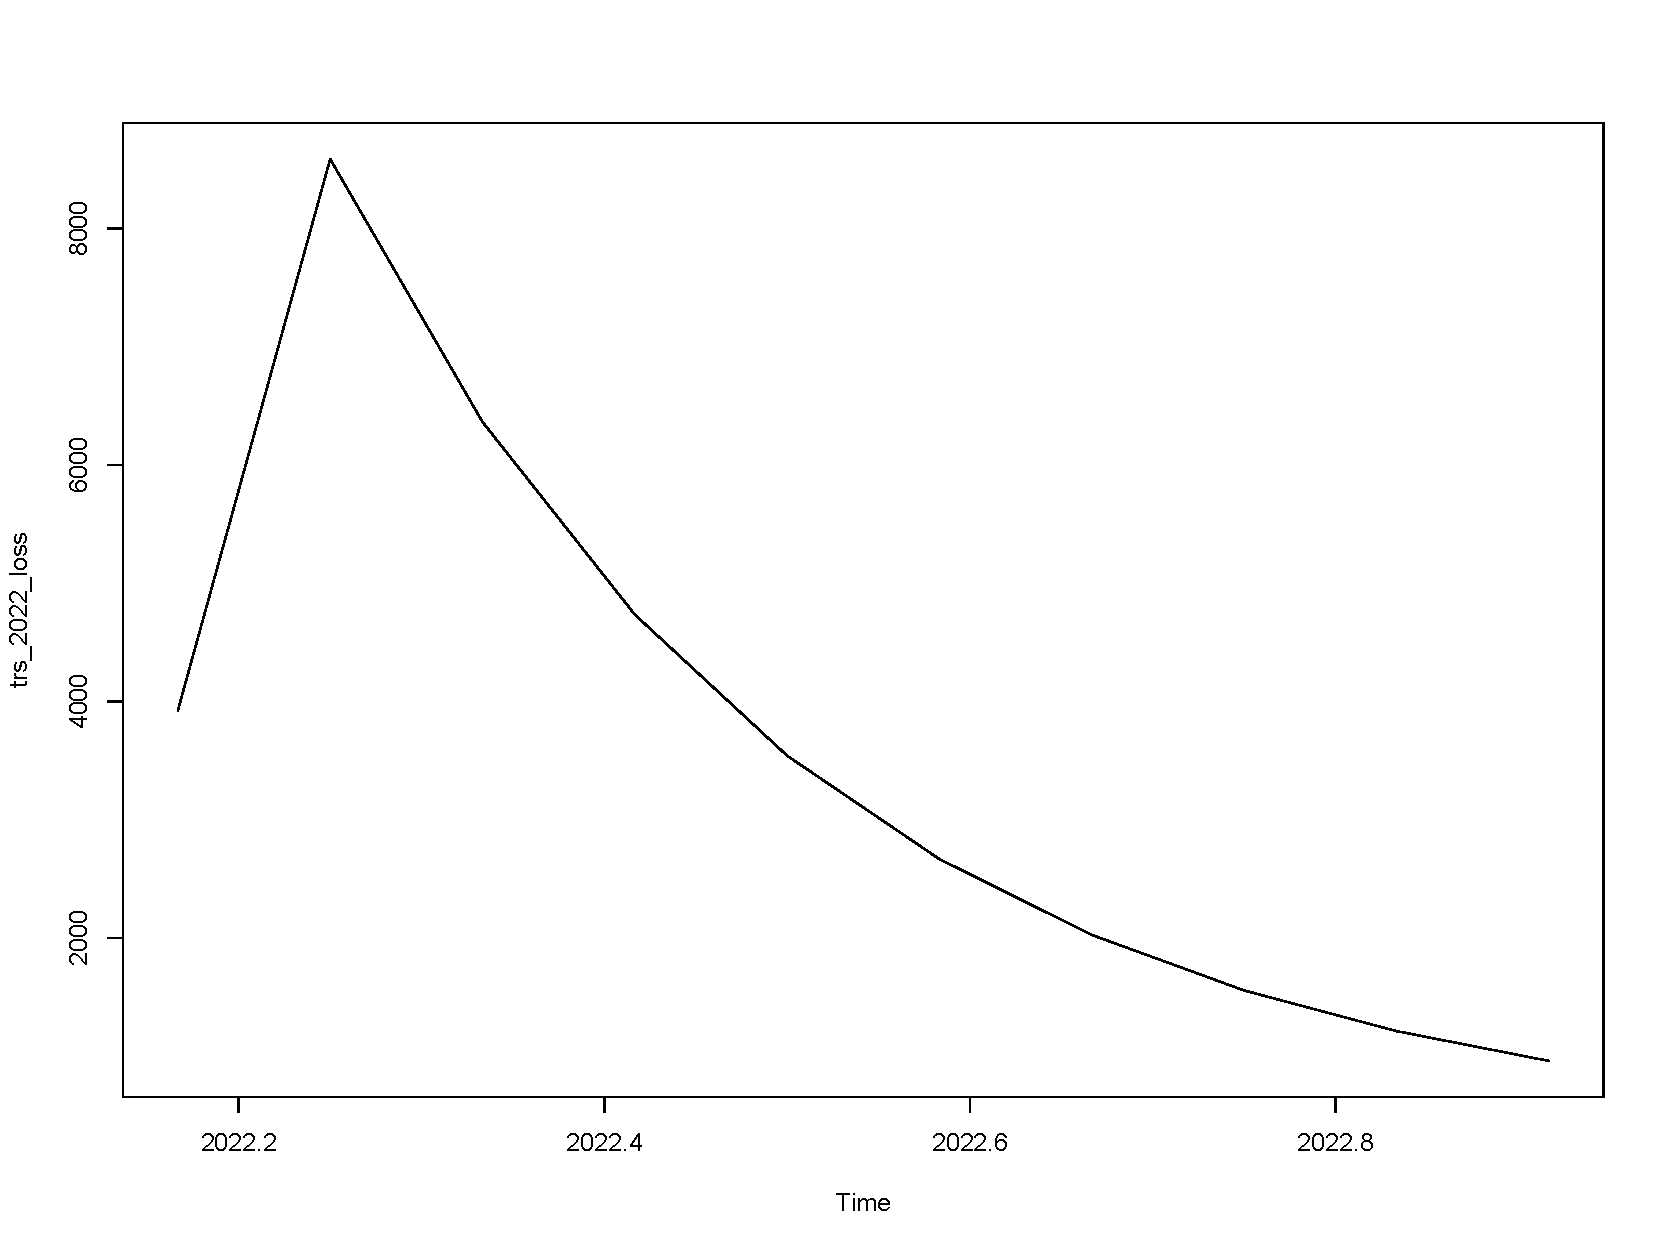
\includegraphics[width=1\textwidth]{figures/loss_2022.pdf} %插入图片,[]中设置图片大小,{}中是图片文件名
      \caption{2022年3月起社会消费品零售总额的损失} %最终文档中希望显示的图片标题
      \label{loss_2022} %用于文内引用的标签
    \end{minipage}
    \begin{minipage}[t]{0.48\textwidth}
      \centering %图片居中
      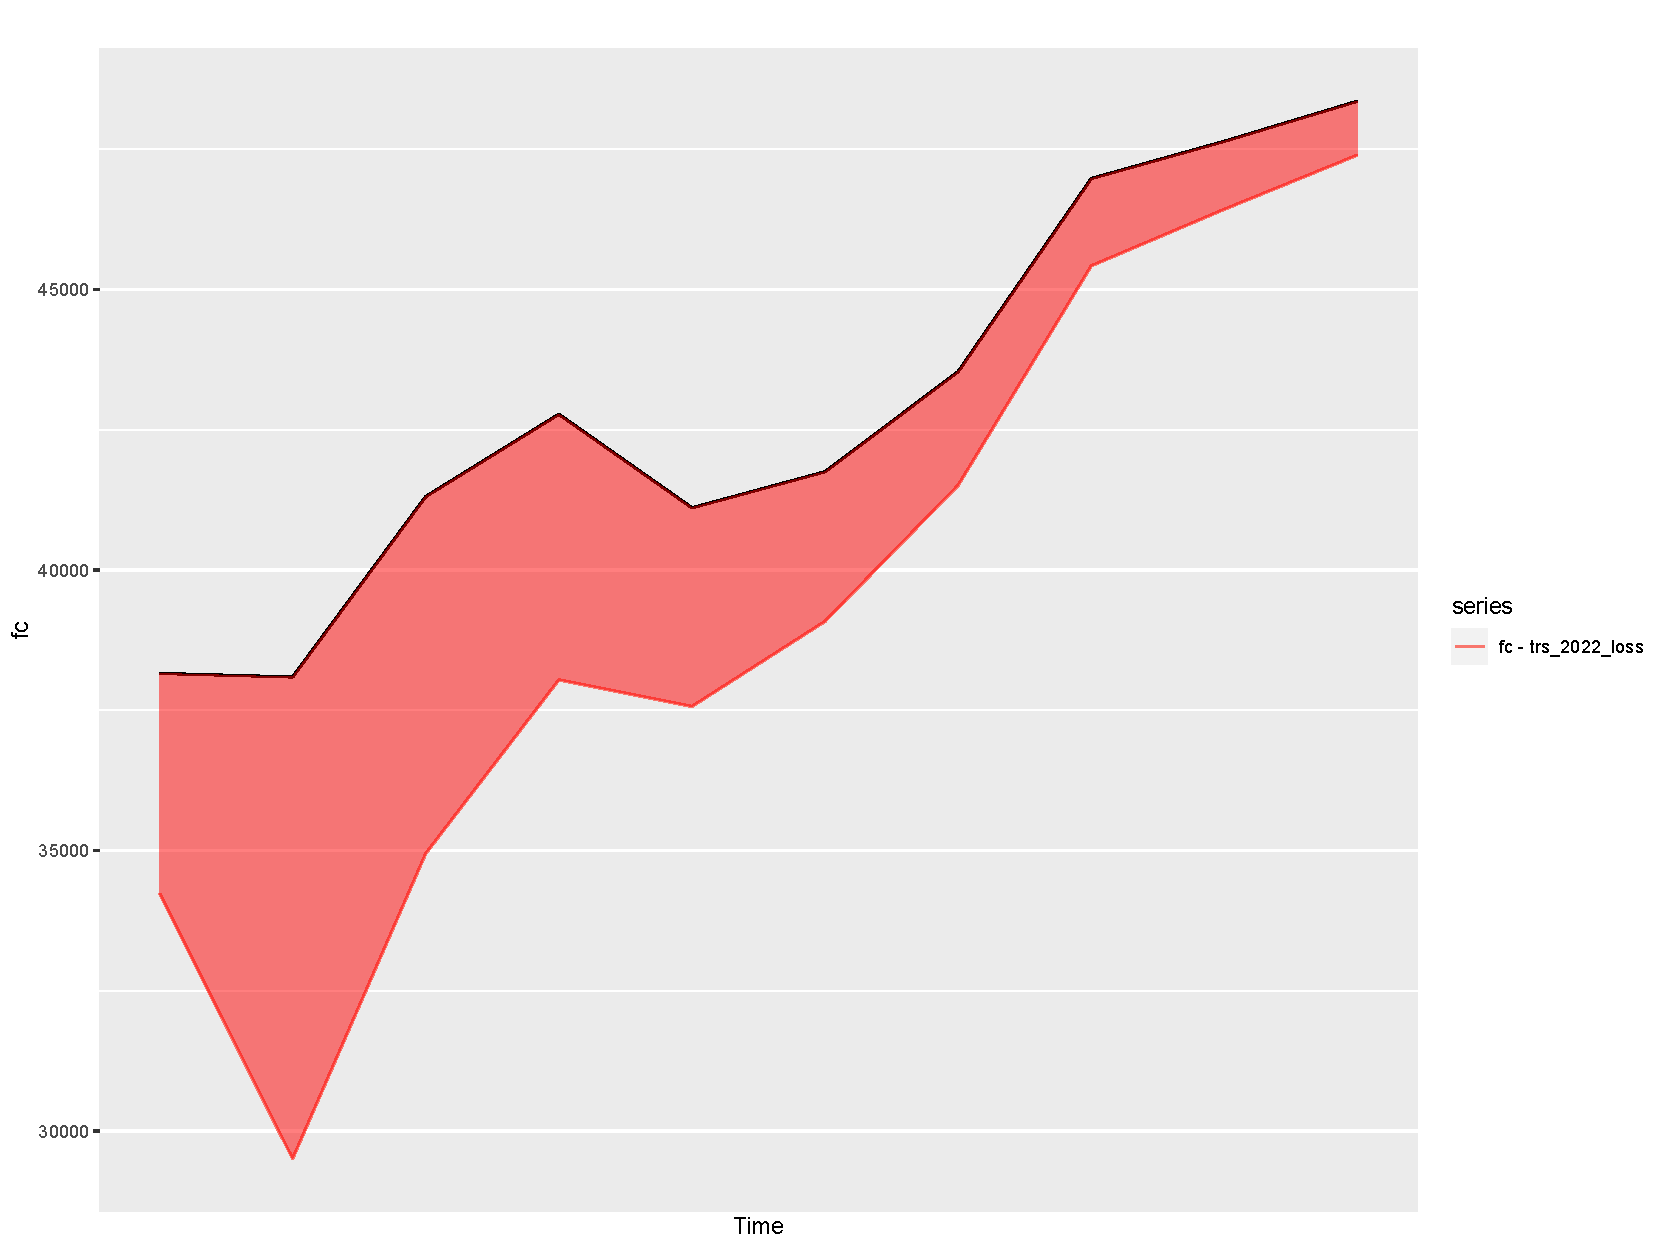
\includegraphics[width=1\textwidth]{figures/compare_2022.pdf} %插入图片,[]中设置图片大小,{}中是图片文件名
      \caption{红色面积为预测损失} %最终文档中希望显示的图片标题
      \label{compare_2022} %用于文内引用的标签
    \end{minipage}
  \end{figure} 
  损失的社会消费品零售总额共计35576.72亿元\nocite{stl}\nocite{yang2022estimating}\nocite{Rob}\nocite{Ruey}\nocite{yandou}
\end{frame}


\begin{frame}{参考文献}
  \bibliographystyle{gbt7714-numerical}
  \bibliography{ref.bib}
\end{frame}
\end{document}